\documentclass[11pt]{article}
\usepackage[margin=0.7in]{geometry}
\usepackage{multirow}
\usepackage {graphicx}
\usepackage[utf8x]{inputenc} % указать кодировку русского текста
\usepackage[russian]{babel} % указать, что язык текста - русский
\usepackage{fancyhdr}
\pagestyle{fancy}
\usepackage{graphicx}
\graphicspath{{pictures/}}
\DeclareGraphicsExtensions{.pdf,.png,.jpg}
\begin{document}
\begin{titlepage}
\begin{center}
\large\textbf{Московский Физико-Технический Институт}\\
\large\textbf{(государственный университет)}
\vfill
\huge\textbf{ Работа 3.3.6}\\
\huge\textbf{Влияние магнитного поля на проводимость полупроводников}\\
\vfill
\large Факультет электроники, фотоники и молекулярной физики\\
\end{center}
\end{titlepage}
\fancyhead[L] {Работа 3.3.6}
\textbf{Цель работы:} Измерение зависомости сопротивления полупроводниковых образцов  различной формы от индукции магнитного поля.\\

\textbf{В работе используются:} электромагнит, миллитесламетр (на основе датчика Холла), вольтметр, амперметр, миллиамперметр, реостат, образцы монокристаллического антимонида индия (InSb) n-типа.\\
\section{Теоретические сведения}:\\
Во внешнем магнитном поле $\vec{B}$ на заряды действует сила Лоренца:
$$\vec{F} = q\vec{E} + q\vec{u}\times \vec{B}$$
Эта сила вызывает движение носителей, которое в общем случае не совпадает с $\vec{E}$. Действительно, траектории частиц будут либо искривляться, либо, если геометрия проводника этого не позволяет, возникнет дополнительное электрическое поле, компенсирующее магнитную составляющую силы Лоренца. Возникновение поперечного току электрического поля в образце, помещенном во внешнее магнитное поле, называют \emph{эффектом Холла}.\\
Для исследования зависимости проводимости среды от магнитного поля используют две основные и принципиально разные по геометрии схемы: мостик Холла и диск Корбино.\\
\indent В схеме с \textbf{мостиком Холла} ток вынуждают течь по оси x вдоль плоской пластинки. Сила Лоренца, действующая со стороны перпендикулярного пластинке магнитного поля, "прибивает" носители заряда к краям образца, что создает холловское электрическое поле, компенсирующее эту силу. Поперечное напряжение между краями пластинки (холловское напряжение) равно $U_{perp} = E_{y}a$, где 
$$E_{y} = \rho_{yx}j_{x} = \frac{j_{x}B}{nq}$$
Таким образом, для холловского напряжения имеем
$$U_{perp} = \frac{B}{nqh}I = R_{H}\frac{B}{h}I$$
$$U_{par} = IR_{0}$$
\indent В схеме \textbf{Корбино} электрическое поле направлено по радиусу системы. В перпендикулярном диску магнитном поле ток вынужден протекать под углом к электрическому полю, то есть линии тока представляют собой спирали. Дополнительное (холловское) электрическое поле при этом не возникает. \\
\indent Ввиду симметрии системы вклад в полный ток даёт только радиальная компонента плотности тока $j_{r} = \sigma_{r}E_{r}$. Полный ток равен $I = 2j_{r}\pi \rho h$, где r - радиус диска, а h - его толщина. Если в системе присутствует один тип носителей, то проводимость в радиальном направлении $\sigma_{r}$ соответствует компоненте $\sigma_{xx}$ тензора:
$$ \sigma_{r} = \frac{\sigma_{0}}{1 + (\mu B)^2}$$
Напряжение между центром и краем диска равно
$$ U = \int E_{r}dr = \frac{\sigma_{r}}{\sigma_{0}}R_{0}I$$
где $R_{0} = \frac{1}{\sigma_{0}2\pi rh}ln\frac{r_{2}}{r_{1}}$ - сопротивление диска в отсутствие магнитного поля. Поэтому закон Ома в схеме Корбино можно записать как
$$ U = IR_{0}(1+(\mu B)^2)$$
Таким образом, в данной схеме появляется зависимость сопротивления образца от магнитного поля. Причина - в геометрии системы: магнитное поле искривляет линии тока, делая их длиннее. Такой эффект называют \emph{геометрическим магнетосопротивлением}.\\
\emph{Магнетосопротивлением} называют зависимость сопротивления образца от величины приложенного магнитного поля.Зависимость R(B) может проявляться только в силу геометрических эффектов, как в примере с диском Корбино. Однако в общем случае магнетосопротивление материалов может быть отлично от нуля и в схеме Холла. Это имеет место, если диагональные компоненты тензора сопротивления зависят от магнитного поля. Это может быть следствием следующих причин:\\
$\rightarrow$ Система является анизотропной и токопроводящие свойства различны в разных направлениях.\\
$\rightarrow$ Система является многокомпонентной. \\
$\rightarrow$ Существуют квантовые эффекты в проводимости, которые приводят к тому, что подвижность зависит от магнитного поля.\\
\textbf{Экспериментальная установка:} Схема установки для исследования магнетосопротивления полупроводников и геометрического резистивного эффекта представлена на рис. 1.\\
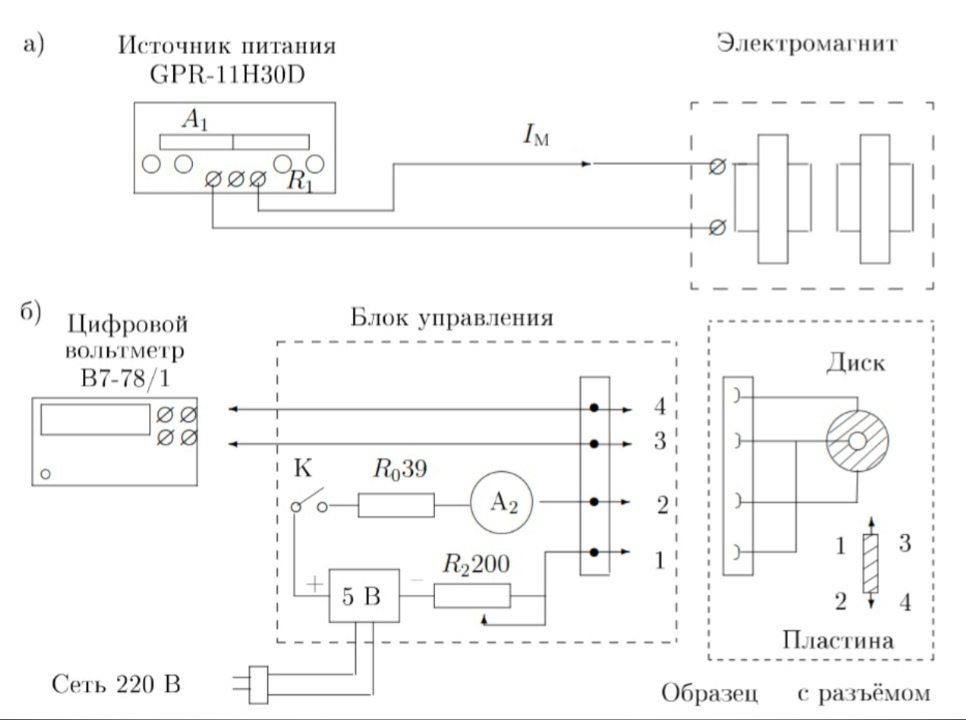
\includegraphics[width = 18cm]{expys}\\

В зазоре электромагнита создаётся постоянное магнитное поле, величину которого можно менять с помощью источника питания электромагнита. Ток электромагнита измеряется амперметром А1. Магнитная индукция в зазоре измеряется с помощью миллитесламетра на основе датчика Холла. \\
Образец в форме кольца (диска Корбино) или пластинки, смонтированный в специальном держателе, подключается к источнику постоянного напряжения 5 В. При замыкании ключа К2 сквозь образец течёт ток, величина которого измеряется миллиамперметром А2 и регулируется реостатом R2. Балластное сопротивление R0 ограничивает ток через образец. Измеряемое напряжение подается на вход вольтметра V.\\
\section{Подготовка}
Диапазон измерения силы тока через образец от 0 до 22,5 mA.\\
Диапазон измерения силы тока через электромагнит от 0 до 0,59 ампер.\\
\section{Калибровка магнита}
С помощью прибора Ш1-10 исследуем зависимость индукции B магнитного поля в зазоре от тока $I_{m}$ через обмотки магнита (для разных полярностей).\\
\\
\begin{tabular}{|l|l|}
\hline
$I_{m}$, амперы, $\sigma_{I} = 0,005$ А & B, mT, $\sigma_{b} = 0,005 mT$\\
\hline
0,01 & 18,1\\
\hline
0,02 & 20,15\\
\hline
0,1 & 101,6\\
\hline
0,2 & 198\\
\hline
0,3 & 280\\
\hline
0,4 & 336\\
\hline
0,45 & 354\\
\hline
0,5 & 368\\
\hline
\end{tabular}
\\
\\
В отсутствии тока $<B> = 9,755$ mT - это значение будет нашим нулём, относительно которого нужно откалибровать все показания. \\
Аппроксимируем по МНК:\\
$ y = kx + b $\\
$ b = <y> - k<x> $\\
$ k = \frac{<yx> - <y><x>}{<x^2> - (<x>)^2} $\\
$ \sigma_{k} = \sqrt{\frac{1}{n-1}(\frac{<y^2> - (<y>)^2}{<x^2> - (<x>)^2} - k^2)} $\\
$ \sigma_{b} = \sigma_{k}\sqrt{<x^2> - (<x>)^2} $\\
$ k = \frac{74,09 - 49,43}{0,093 - 0,06} \approx 747,3 $\\
$ \sigma_{k} = \sqrt{\frac{1}{7}(\frac{58795,2 - 39890}{0,093 - 0,06} - 747,3^2)}  \approx 45,4 $\\
$ b = 199,7 - 747,3 \times 0,24 \approx 12,9$ mT\\
$ \sigma_{b} = 45,4\sqrt{0,093 - 0,06} \approx 8,2 $\\
Итоговая аппроксимирующая прямая имеет вид: \fbox{$y = 747,3x + 12,9$}\\
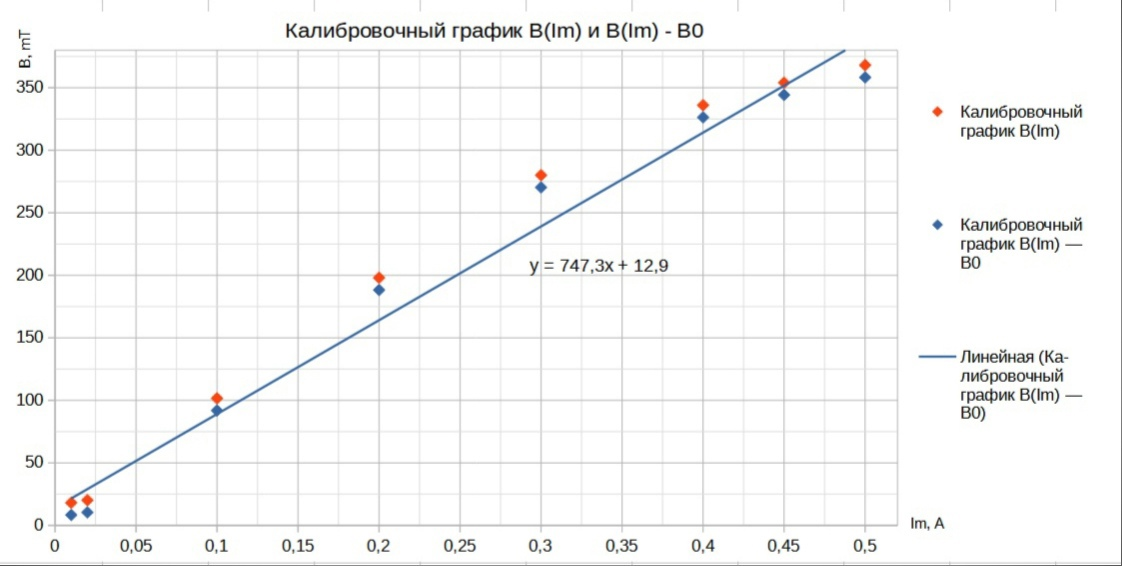
\includegraphics[width = 18cm]{graph1}\\
\section{Снятие показаний}
\textbf{1)} Подключим диск Корбино к электрической цепи.При помощи реостата R2 установим ток через образец $I_{0} = 22,5$ mA. Падение напряжения на образце в отсутствие магнитного поля $U = 0,715$ mV. \\
Вставим держатель с диском в зазор электромагнита. Снимем зависимость напряжения U на образце от тока $I_{m}$ через обмотки магнита при фиксированном токе через образец $I_{0} = 22,5$ mA:\\
\\
\begin{tabular}{|l|l|l|}
\hline
$I_{m}$, ампер, $\sigma_{I} = 0,005$ ампер & U, mV, $\sigma_{U}$ = 0,0005 mV & $U_{down}$, mV, $\sigma_{U}$ = 0,0005 mV \\
\hline
0,01 & 0,716 & 0,710\\
\hline
0,03 & 0,730 & 0,727\\
\hline
0,07 & 0,831 & 0,832\\
\hline
0,1 & 0,972 & 0,976\\
\hline
0,14 & 1,148 & 1,176\\
\hline
0,17 & 1,351 & 1,388\\
\hline
0,2 & 1,568 & 1,585\\
\hline
0,25 & 1,916 & 2,008\\
\hline
0,28 & 2,240 & 2,286\\
\hline
0,3 & 2,358 & 2,445\\
\hline
0,33 & 2,558 & 2,694\\
\hline
0,37 & 2,805 & 2,866\\
\hline
0,4 & 2,960 & 3,020\\
\hline
0,44 & 3,105 & 3,137\\
\hline
0,47 & 3,220 & 3,230\\
\hline
0,51 & 3,310 & 3,333\\
\hline
0,55 & 3,413 & 3,400\\
\hline
\end{tabular}
\\
\\

То же самое проделаем для остальных измерений.\\
Пластина, ширина вдоль поля:\\
$I_{0} = 10 mA$, падение напряжения в отсутствии магнитного поля $U = 0,727$ mA\\
\\
\begin{tabular}{|l|l|l|}
\hline
$I_{m}$, ампер, $\sigma_{I} = 0,005$ ампер & U, mV, $\sigma_{U}$ = 0,0005 mV & $U_{down}$, mV, $\sigma_{U}$ = 0,0005 mV \\
\hline
0,01 & 0,726 & 0,724\\
\hline
0,05 & 0,734 & 0,733\\
\hline 
0,08 & 0,751 & 0,748\\
\hline
0,12 & 0,774 & 0,776\\
\hline
0,15 & 0,800 & 0,802\\
\hline
0,18 & 0,830 & 0,829\\
\hline
0,22 & 0,858 & 0,861\\
\hline
0,25 & 0,887 & 0,887\\
\hline
0,29 & 0,915 & 0,920\\
\hline
0,33 & 0,948 & 0,950\\
\hline
0,37 & 0,973 & 0,972\\
\hline
0,41 & 0,988 & 0,987\\
\hline
0,45 & 1,002 & 0,998\\
\hline
0,48 & 1,011 & 1,004\\
\hline
0,51 & 1,020 & 1,011\\
\hline
0,55 & 1,030 & 1,018\\
\hline
\end{tabular}
\\
\\
Пластина, ширина поперек поля:\\
$I_{0} = 10 mA$, падение напряжения в отсутствии магнитного поля $U = 0,720$ mA\\
\\
\begin{tabular}{|l|l|l|}
\hline
$I_{m}$, ампер, $\sigma_{I} = 0,005$ ампер & U, mV, $\sigma_{U}$ = 0,0005 mV & $U_{down}$, mV, $\sigma_{U}$ = 0,0005 mV \\
\hline
0,01 & 0,721 & 0,720\\
\hline
0,05 & 0,745 & 0,750\\
\hline
0,08 & 0,784 & 0,788\\
\hline
0,12 & 0,850 & 0,863\\
\hline
0,15 & 0,909 & 0,920\\
\hline
0,18 & 0,977 & 0,997\\
\hline
0,22 & 1,055 & 1,068\\
\hline
0,25 & 1,122 & 1,135\\
\hline
0,29 & 1,205 & 1,220\\
\hline
0,33 & 1,276 & 1,296\\
\hline
0,37 & 1,336 & 1,344\\
\hline
0,41 & 1,372 & 1,382\\
\hline
0,45 & 1,407 & 1,414\\
\hline
0,48 & 1,432 & 1,430\\
\hline
0,51 & 1,447 & 1,444\\
\hline
0,55 & 1,468 & 1,464\\
\hline
\end{tabular}
\\
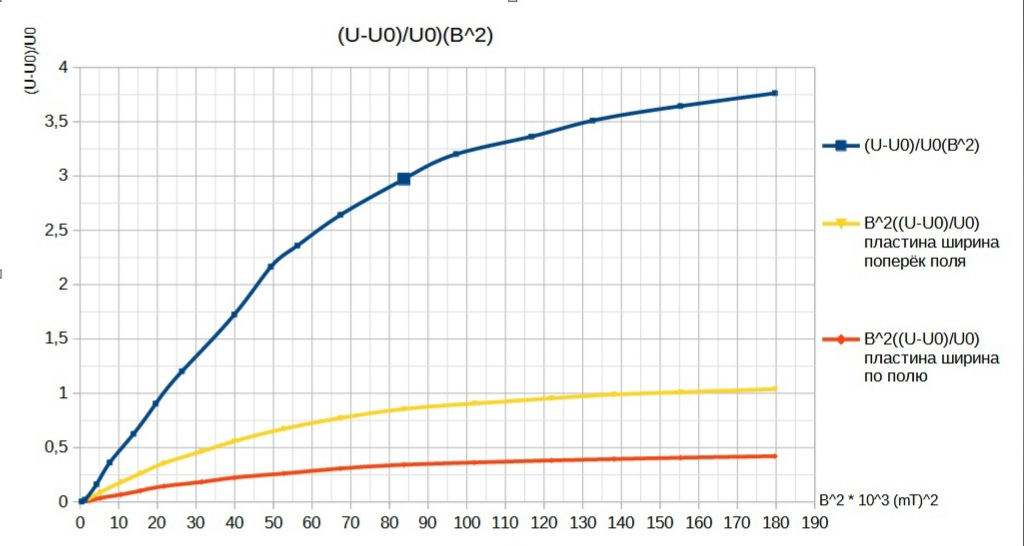
\includegraphics[width = 19cm]{graph2}\\
\\
\textbf{2)} Используя формулу $ U = IR_{0}(1+(\mu B)^2)$ построим график зависимости $\frac{U - U_{0}}{U_{0}}(B^2)$, по наклону которого для прямолинейного участка измерений для диска Корбино можно будет рассчитать подвижность носителей.\\
Прямолинейный участок сделаем путём аппроксимирования первых значений (вблизи нуля, где всё еще почти линейно) МНК.\\
$ y = kx + b $\\
$ b = <y> - k<x> $\\
$ k = \frac{<yx> - <y><x>}{<x^2> - (<x>)^2} $\\
$ \sigma_{k} = \sqrt{\frac{1}{n-1}(\frac{<y^2> - (<y>)^2}{<x^2> - (<x>)^2} - k^2)} $\\
$ \sigma_{b} = \sigma_{k}\sqrt{<x^2> - (<x>)^2} $\\
$ k = \frac{16,29 - 8,85}{367,4 - 200,2} \approx 0,044 $\\
$ \sigma_{k} = \sqrt{\frac{1}{7}(\frac{0,72 - 0,39}{367,4 - 200,2} - 0,044^2)}  \approx 0,002 $\\
$ b = 0,626 - 0,044 \times 14,15 \approx -0,005$ \\
$ \sigma_{b} = 0,002\sqrt{367,4 - 200,2} \approx 0,03 $\\
Итоговая аппроксимирующая прямая имеет вид: \fbox{$y = 0,044x - 0,005$}\\
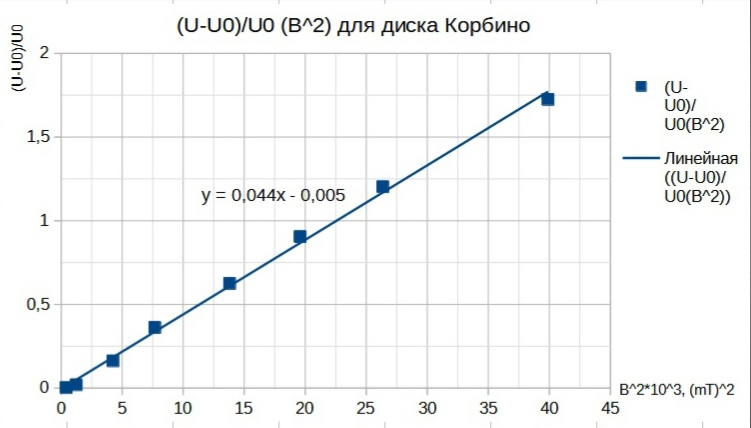
\includegraphics[width=19cm]{graph3}\\
\\
\textbf{3)} $(\mu)^2 = \frac{U - U_{0}}{U_{0}B^2} $.\\ Для графика в наших координатах $(\mu)^2 = \frac{dy}{dx}$, поэтому $\mu = \sqrt{\frac{dy}{dx}}$\\
$\frac{dy}{dx} = 0,044 \times 10^3 $, следовательно, $\mu \approx 6,6 \frac{m^2}{V * c}$  \\
Табличное значение подвижности InSb: $\mu_{InSb} = 7.7 \frac{m^2}{V * c}$\\
Таким образом, подвижность была измерена с погрешностью 14$\%$.\\
\\
\textbf{4)} Определим сопротивление диска $R_{0}$ в отсутствие магнитного поля:\\
$R_{0} = \frac{U_{0}}{I_{0}} = \frac{0,715 mV}{22,5 mA} \approx 0,03$ Ом.\\
$(\frac{\sigma_{R_{0}}}{R_{0}})^2 = (\frac{\sigma_{U_{0}}}{U_{0}})^2 + (\frac{\sigma_{I_{0}}}{I_{0}})^2$\\
$(\frac{\sigma_{R_{0}}}{R_{0}})^2 = (\frac{1}{22,5})^2 + (\frac{0,0005}{0,715})^2 \approx (\frac{1}{22,5})^2$\\
$\sigma_{R_{0}} \approx 0,001$ Ом.\\
\textbf{5)} Рассчитаем концентрацию носителей тока n, удельное сопротивление $\rho_{0}$ и удельную проводимость $\sigma_{0} = 1/\rho_{0}$ материала образца.\\
$R_{0} = \frac{1}{\sigma_{0}2\pi rh}ln(\frac{r_{2}}{r_{1}})$\\
$\sigma_{0} \approx 0,528 \pm 0,007 \frac{1}{Om * m}$\\
$\rho_{0} = 1/\sigma_{0} \approx 18,9 \pm 0,3 \frac{Om * (mm)^2}{m}$\\
 

\section{Вывод}
Мы измерили концентрацию носителей заряда и их подвижность для антимонида индия. Значения подвижности частиц для InSb получились с погрешностью 14$\%$ относительно табличных.\\
\end{document}